% ============================================================
% UZYNTRA Security - Company Overview Document
% Compile from repository root with: pdflatex UZYNTRA-Company-Overview.tex
% Logo used: public/logos/uzyntra-pdf-logo.png
% ============================================================
\documentclass[11pt,a4paper]{article}

\usepackage[T1]{fontenc}
\usepackage[utf8]{inputenc}
\usepackage{lmodern}
\usepackage[margin=2.05cm,top=2.25cm,bottom=2.45cm,headheight=16pt,headsep=0.65cm,footskip=1.1cm]{geometry}
\usepackage[table]{xcolor}
\usepackage{graphicx}
\usepackage[explicit]{titlesec}
\usepackage{enumitem}
\usepackage{tabularx}
\usepackage{booktabs}
\usepackage{array}
\usepackage{parskip}
\usepackage{microtype}
\usepackage{fancyhdr}
\usepackage{hyperref}
\usepackage{mdframed}
\usepackage{multicol}
\usepackage{needspace}
\usepackage{tikz}

\setcounter{secnumdepth}{0}
\raggedbottom
\sloppy
\emergencystretch=2em

% Brand colours
\definecolor{uzred}{HTML}{EF1F24}
\definecolor{uzreddeep}{HTML}{991B1B}
\definecolor{uzredsoft}{HTML}{FEF2F2}
\definecolor{uzink}{HTML}{070708}
\definecolor{uzpanel}{HTML}{111114}
\definecolor{uzslate}{HTML}{0F172A}
\definecolor{uzgray}{HTML}{475569}
\definecolor{uzmuted}{HTML}{64748B}
\definecolor{uzline}{HTML}{E2E8F0}
\definecolor{uzcard}{HTML}{F8FAFC}

\hypersetup{
  colorlinks=true,
  linkcolor=uzred,
  urlcolor=uzred,
  pdftitle={UZYNTRA Security - Company Overview},
  pdfauthor={UZYNTRA Security},
  pdfsubject={Services, Products, Courses, and Engagement Overview},
}

% Typography and heading protection
\titleformat{\section}
  {\Needspace{8\baselineskip}\sffamily\Large\bfseries\color{uzslate}}
  {}
  {0pt}
  {\noindent\colorbox{uzredsoft}{\parbox{\dimexpr\linewidth-2\fboxsep\relax}{\strut\textcolor{uzred}{\small\MakeUppercase{#1}}\strut}}\par\vspace{4pt}\textcolor{uzred}{\rule{\linewidth}{1.1pt}}\vspace{2pt}}

\titleformat{\subsection}
  {\Needspace{5\baselineskip}\sffamily\large\bfseries\color{uzslate}}
  {}
  {0pt}
  {#1\par\vspace{-2pt}\textcolor{uzline}{\rule{\linewidth}{0.55pt}}}

\titlespacing*{\section}{0pt}{18pt}{10pt}
\titlespacing*{\subsection}{0pt}{14pt}{6pt}

% Header / footer
\pagestyle{fancy}
\fancyhf{}
\renewcommand{\headrulewidth}{0pt}
\fancyhead[L]{\small\sffamily\color{uzgray}\textbf{UZYNTRA Security} / Confidential Company Overview}
\fancyhead[R]{\small\sffamily\color{uzgray}\thepage}
\fancyfoot[C]{\small\sffamily\color{uzgray}%
  \href{https://uzyntra.com}{uzyntra.com}\quad | \quad
  \href{mailto:security@uzyntra.com}{security@uzyntra.com}\quad | \quad
  +92 333 5545728}

\newmdenv[
  linecolor=uzred,
  linewidth=1.1pt,
  leftline=true,rightline=false,topline=false,bottomline=false,
  backgroundcolor=uzredsoft,
  innerleftmargin=11pt,innerrightmargin=10pt,innertopmargin=8pt,innerbottommargin=8pt,
  skipabove=7pt,skipbelow=9pt
]{redbar}

\newmdenv[
  linecolor=uzline,
  linewidth=0.75pt,
  backgroundcolor=uzcard,
  innerleftmargin=11pt,innerrightmargin=11pt,innertopmargin=10pt,innerbottommargin=10pt,
  skipabove=7pt,skipbelow=9pt,
  roundcorner=5pt
]{infobox}

\newcommand{\metriccard}[2]{%
  \fcolorbox{white!18}{white!7}{\begin{minipage}[t][2.45cm][c]{0.205\linewidth}\centering\sffamily\textcolor{white!55}{\scriptsize\MakeUppercase{#1}}\par\vspace{4pt}\textcolor{white}{\bfseries #2}\end{minipage}}%
}

\newcommand{\contactline}{%
  \href{https://uzyntra.com}{uzyntra.com}\quad | \quad
  \href{mailto:security@uzyntra.com}{security@uzyntra.com}\quad | \quad
  +92 333 5545728}

\setlist[itemize]{
  leftmargin=1.35em,
  itemsep=3pt,
  topsep=4pt,
  parsep=0pt,
  label={\textcolor{uzred}{\small$\bullet$}}
}

\begin{document}

% Cover
\begin{titlepage}
\thispagestyle{empty}
\newgeometry{margin=0cm}
\pagecolor{uzink}
\begin{tikzpicture}[remember picture,overlay]
  \fill[uzink] (current page.south west) rectangle (current page.north east);
  \fill[uzreddeep] (current page.north east) ++(-4.8cm,0) rectangle (current page.south east);
  \fill[uzred,opacity=0.92] (current page.north west) rectangle ++(0.42cm,-\paperheight);
  \draw[white,opacity=0.05,step=1.05cm] (current page.south west) grid (current page.north east);
  \fill[uzred,opacity=0.18] ([xshift=-6cm,yshift=-2cm]current page.north east) circle (5.5cm);
  \fill[uzred,opacity=0.10] ([xshift=2cm,yshift=1cm]current page.south west) circle (6cm);
\end{tikzpicture}

\vspace*{2cm}
\hspace*{1.6cm}\begin{minipage}{0.76\linewidth}
  
\includegraphics[height=1.8cm,keepaspectratio]{public/logos/uzyntra-pdf-logo.png}\hspace{0.45cm}%
  \raisebox{0.43cm}{\sffamily\bfseries\Large\textcolor{white}{UZYNTRA Security}}

  \vspace{2.0cm}
  {\sffamily\bfseries\fontsize{38}{44}\selectfont\textcolor{white}{Company Overview}}\par
  \vspace{0.35cm}
  {\sffamily\bfseries\Large\textcolor{uzred}{Services / Products / Courses}}\par
  \vspace{0.8cm}
  {\sffamily\large\textcolor{white!72}{Enterprise cybersecurity, secure software engineering, blockchain systems, and production-ready security technology.}}\par

  \vspace{1.35cm}
  \textcolor{uzred}{\rule{0.72\linewidth}{1.4pt}}\par
  \vspace{0.9cm}
  \metriccard{Security}{Offensive testing}\hfill
  \metriccard{Engineering}{Secure systems}\hfill
  \metriccard{Product}{API Firewall}\hfill
  \metriccard{Training}{Professional labs}

  \vfill
  {\sffamily\small\textcolor{white!62}{Confidential overview prepared for business, product, and training discussions.}}\par
  \vspace{0.35cm}
  {\sffamily\small\textcolor{white!52}{\contactline}}\par
  \vspace{0.25cm}
  {\sffamily\footnotesize\textcolor{white!42}{\href{https://github.com/UZYNTRA-Security}{github.com/UZYNTRA-Security}}}
\end{minipage}
\restoregeometry
\end{titlepage}
\pagecolor{white}

\clearpage
\thispagestyle{fancy}
\tableofcontents
\clearpage

\section{About UZYNTRA Security}

\begin{redbar}
\textbf{UZYNTRA Security} is a platform and services company delivering enterprise-grade cybersecurity solutions, secure software engineering, and blockchain systems built with modern architecture, security-first thinking, and production-ready technology.
\end{redbar}

UZYNTRA Security operates at the intersection of offensive security, secure engineering, and emerging technology. The company serves organisations that need both the expertise to identify and eliminate vulnerabilities and the engineering capability to build systems that are secure by design.

\subsection{Mission}
To help organisations build, protect, and scale secure digital systems through cybersecurity, secure software development, and blockchain engineering.

\subsection{Core Positioning}
UZYNTRA Security is not a single-product vendor. It is a full-spectrum security and engineering platform offering:
\begin{itemize}
  \item Offensive security services: API testing, penetration testing, and red teaming.
  \item Secure engineering services: backend, cloud, blockchain, and automation systems.
  \item A flagship open-source security product: UZYNTRA API Firewall Platform.
  \item Professional training and exclusive certification programmes.
\end{itemize}

\begin{infobox}
\textbf{Primary contact:} \href{mailto:security@uzyntra.com}{security@uzyntra.com}\quad
\textbf{Phone:} +92 333 5545728\quad
\textbf{Web:} \href{https://uzyntra.com}{uzyntra.com}
\end{infobox}

\section{Services}
UZYNTRA Security offers five core service lines, each designed to address a distinct dimension of enterprise security and engineering.

\subsection{API \& SaaS Security Testing}
\begin{redbar}\textit{Offensive testing for APIs, SaaS platforms, authentication systems, and cloud services.}\end{redbar}
UZYNTRA identifies exploitable vulnerabilities in APIs, authentication flows, and SaaS attack surfaces before adversaries do, using OWASP methodology and real-world abuse scenarios.

\textbf{Coverage areas:}
\begin{multicols}{2}
\begin{itemize}
  \item OWASP API Top 10
  \item BOLA / IDOR
  \item JWT, OAuth 2.0, and API key abuse
  \item Business logic and privilege escalation
  \item Rate limiting and mass assignment
  \item SaaS tenant isolation
  \item Cloud-connected API enumeration
  \item Injection and validation flaws
\end{itemize}
\end{multicols}
\textbf{Deliverable:} Detailed security report with CVSS-scored findings, proof-of-concept evidence, and remediation guidance.

\subsection{Penetration Testing \& Red Teaming}
\begin{redbar}\textit{Real-world attack simulations across infrastructure, applications, and identity systems.}\end{redbar}
\begin{tabularx}{\linewidth}{@{}>{\bfseries}p{0.31\linewidth}X@{}}
\toprule
Type & Description \\
\midrule
Web Application Pentest & OWASP Top 10, business logic, authentication, and session management. \\
Network \& Infrastructure & Internal and external network testing, firewall bypass, and lateral movement. \\
Cloud Security Assessment & AWS, Azure, and GCP misconfiguration review plus IAM escalation paths. \\
Identity \& Active Directory & Kerberoasting, pass-the-hash, domain privilege escalation, and identity abuse. \\
Red Team Operation & Full adversary simulation with defined objectives and realistic TTPs. \\
\bottomrule
\end{tabularx}

\subsection{Secure Backend \& Cloud Engineering}
\begin{redbar}\textit{Design and development of secure backend systems, APIs, and cloud-native architectures.}\end{redbar}
\begin{itemize}
  \item Rust-based high-performance backend and API development.
  \item Secure REST and GraphQL API design with authentication and authorisation.
  \item Cloud-native architecture on AWS, Azure, and GCP.
  \item DevSecOps pipeline integration: SAST, DAST, SCA, and IaC scanning.
  \item Infrastructure as Code with Terraform and Pulumi.
  \item Container security for Docker, Kubernetes, Helm, and deployment hardening.
\end{itemize}

\subsection{Blockchain Security \& Smart Contract Engineering}
\begin{redbar}\textit{Smart contract development, blockchain security reviews, dApp architecture, and Web3 engineering.}\end{redbar}
\begin{itemize}
  \item Solidity smart contract development and security review.
  \item DeFi protocol architecture and vulnerability assessment.
  \item dApp frontend and backend integration with Ethers.js and Wagmi.
  \item ERC-20, ERC-721, ERC-1155 token systems and token economics.
  \item Multi-chain deployment across Ethereum, Polygon, and Solana.
  \item Wallet integration, secure key management, IPFS, and decentralised storage.
\end{itemize}

\subsection{Automation \& AI Workflow Systems}
\begin{redbar}\textit{n8n automation, API orchestration, AI pipelines, and self-hosted workflow systems.}\end{redbar}
\begin{itemize}
  \item n8n self-hosted workflow design, deployment, and maintenance.
  \item API orchestration and webhook-driven event pipelines.
  \item LangChain and LlamaIndex agent workflow construction.
  \item Multi-agent system design with tool use and memory.
  \item Secure automation with credential management and audit logging.
  \item Integration with CRMs, ERPs, communication platforms, and databases.
\end{itemize}

\section{Product: UZYNTRA API Firewall Platform}
\begin{redbar}
\textbf{Flagship open-source security product.} A high-performance Rust API security engine unified with a Next.js operator control console for real-time request inspection, threat detection, active mitigation, telemetry, and policy control.
\end{redbar}

\subsection{Platform Architecture}
\begin{tabularx}{\linewidth}{@{}>{\bfseries}p{0.28\linewidth}X@{}}
\toprule
Component & Description \\
\midrule
Rust Security Engine & High-performance async reverse-proxy firewall built with Tokio, Axum, Reqwest, and Serde. It sits between clients and backend services. \\
Next.js Operator Console & Modern SaaS-style control plane for monitoring, investigation, mitigation management, audit review, and policy control. \\
\bottomrule
\end{tabularx}

\begin{infobox}
\centering\sffamily\small\texttt{Client -> UZYNTRA Firewall -> Inspection -> Detection -> Decision -> Backend}
\end{infobox}

\subsection{Rust Engine Capabilities}
\begin{tabularx}{\linewidth}{@{}>{\bfseries}p{0.30\linewidth}X@{}}
\toprule
Capability & Detail \\
\midrule
Deep Request Inspection & Analyse headers, query strings, routes, payloads, and request context before traffic reaches the backend. \\
Attack Detection Engine & Pattern matching, heuristic scoring, confidence levels, and attack classification for API threats. \\
Active Mitigation & Block malicious requests, apply TTL bans, reset reputation, and enforce decisions through the proxy layer. \\
Security Telemetry & Emit events, metrics, logs, routes, severity, attack types, and actions for operational review. \\
Policy Control & Manage rules, rate limiting, and enforcement behaviour through admin APIs and the operator console. \\
High Performance & Built with Tokio, Axum, Reqwest, and Serde for async Rust throughput and predictable latency. \\
\bottomrule
\end{tabularx}

\subsection{Operator Control Console}
\begin{tabularx}{\linewidth}{@{}>{\bfseries}p{0.30\linewidth}X@{}}
\toprule
Module & Function \\
\midrule
Dashboard & Live metrics, attack activity, security posture, and operational health. \\
Events Explorer & Search, filter, and investigate attack events with route, IP, severity, and attack context. \\
Mitigation Control & Review blocked traffic, TTL bans, IP reputation changes, and response decisions. \\
Reputation System & Track source behaviour and reputation signals for repeated abuse control. \\
Audit Trail & Review operator actions, policy changes, and security events for accountability. \\
Policy Management & Tune security policies and control firewall behaviour from a modern SaaS-style console. \\
\bottomrule
\end{tabularx}

\subsection{Detection Coverage and Use Cases}
\begin{multicols}{2}
\begin{itemize}
  \item SQL Injection
  \item Cross-Site Scripting
  \item Path Traversal
  \item Rate Abuse
  \item Behavioural Anomalies
  \item API security platforms
  \item Reverse proxy security
  \item DevSecOps pipelines
  \item SaaS backend protection
  \item SIEM-ready telemetry workflows
\end{itemize}
\end{multicols}

\subsection{Technical Stack}
\begin{infobox}
\begin{tabularx}{\linewidth}{@{}>{\bfseries}p{0.28\linewidth}X@{}}
Engine & Rust, Tokio, Axum, Reqwest, Serde \\
Control Plane & Next.js App Router, Tailwind CSS, REST API integration \\
Deployment & Docker, GitHub Actions, cloud-native services \\
Observability & JSON logs, events, metrics, audit records, SIEM-ready output \\
Proxy & \texttt{http://127.0.0.1:8080} \\
Admin API & \texttt{http://127.0.0.1:9090} \\
\end{tabularx}
\end{infobox}

\subsection{Open Source Repositories}
\begin{infobox}
\begin{tabularx}{\linewidth}{@{}>{\bfseries}p{0.28\linewidth}X@{}}
Firewall Engine & \href{https://github.com/UsamaMatrix/uzyntra-api-firewall}{github.com/UsamaMatrix/uzyntra-api-firewall} \\
Operator UI & \href{https://github.com/UsamaMatrix/uzyntra-ui}{github.com/UsamaMatrix/uzyntra-ui} \\
Organisation & \href{https://github.com/UZYNTRA-Security}{github.com/UZYNTRA-Security} \\
\end{tabularx}
\end{infobox}

\section{Professional Training Programmes}
\begin{tabularx}{\linewidth}{@{}>{\bfseries}p{0.26\linewidth}p{0.18\linewidth}p{0.20\linewidth}X@{}}
\toprule
Programme & Duration & Fee & Focus \\
\midrule
Cybersecurity Professional Programme & 3 Months & PKR 45,000 / \$199 USD & Security foundations, vulnerability assessment, pentesting fundamentals, monitoring, incident response, and reporting. \\
AI Professional Programme & 3 Months & PKR 54,000 / \$249 USD & Python, ML, deep learning, LLMs, AI agents, MLOps, deployment, and responsible AI. \\
\bottomrule
\end{tabularx}

\section{Contact \& Engagement}
\begin{infobox}
\begin{tabularx}{\linewidth}{@{}>{\bfseries}p{0.24\linewidth}X@{}}
Website & \href{https://uzyntra.com}{https://uzyntra.com} \\
Email & \href{mailto:security@uzyntra.com}{security@uzyntra.com} \\
Phone & +92 333 5545728 \\
GitHub & \href{https://github.com/UZYNTRA-Security}{github.com/UZYNTRA-Security} \\
LinkedIn & \href{https://linkedin.com/company/uzyntra}{linkedin.com/company/uzyntra} \\
X / Twitter & \href{https://x.com/uzyntra}{x.com/uzyntra} \\
Instagram & \href{https://instagram.com/uzyntra}{instagram.com/uzyntra} \\
\end{tabularx}
\end{infobox}

To engage UZYNTRA Security for a service, product deployment, or training enquiry, reach out via email or the contact form at \href{https://uzyntra.com/contact}{uzyntra.com/contact}.

\vfill
\begin{center}
\textcolor{uzline}{\rule{0.48\linewidth}{0.5pt}}\\[7pt]
{\small\sffamily\color{uzgray}\textcopyright{} UZYNTRA Security. All rights reserved. \href{https://uzyntra.com}{uzyntra.com}}
\end{center}

\end{document}
